\documentclass{beamer}
\mode<presentation>
\usepackage{amsmath,amssymb,mathtools}
\usepackage{textcomp}
\usepackage{gensymb}
\usepackage{adjustbox}
\usepackage{subcaption}
\usepackage{enumitem}
\usepackage{multicol}
\usepackage{listings}
\usepackage{url}
\usepackage{graphicx} % <-- needed for images
\def\UrlBreaks{\do\/\do-}

\usetheme{Boadilla}
\usecolortheme{lily}
\setbeamertemplate{footline}{
  \leavevmode%
  \hbox{%
  \begin{beamercolorbox}[wd=\paperwidth,ht=2ex,dp=1ex,right]{author in head/foot}%
    \insertframenumber{} / \inserttotalframenumber\hspace*{2ex}
  \end{beamercolorbox}}%
  \vskip0pt%
}
\setbeamertemplate{navigation symbols}{}

\lstset{
  frame=single,
  breaklines=true,
  columns=fullflexible,
  basicstyle=\ttfamily\tiny   % tiny font so code fits
}

\numberwithin{equation}{section}

% ---- your macros ----
\providecommand{\nCr}[2]{\,^{#1}C_{#2}}
\providecommand{\nPr}[2]{\,^{#1}P_{#2}}
\providecommand{\mbf}{\mathbf}
\providecommand{\pr}[1]{\ensuremath{\Pr\left(#1\right)}}
\providecommand{\qfunc}[1]{\ensuremath{Q\left(#1\right)}}
\providecommand{\sbrak}[1]{\ensuremath{{}\left[#1\right]}}
\providecommand{\lsbrak}[1]{\ensuremath{{}\left[#1\right.}}
\providecommand{\rsbrak}[1]{\ensuremath{\left.#1\right]}}
\providecommand{\brak}[1]{\ensuremath{\left(#1\right)}}
\providecommand{\lbrak}[1]{\ensuremath{\left(#1\right.}}
\providecommand{\rbrak}[1]{\ensuremath{\left.#1\right)}}
\providecommand{\cbrak}[1]{\ensuremath{\left\{#1\right\}}}
\providecommand{\lcbrak}[1]{\ensuremath{\left\{#1\right.}}
\providecommand{\rcbrak}[1]{\ensuremath{\left.#1\right\}}}
\theoremstyle{remark}
\newtheorem{rem}{Remark}
\newcommand{\sgn}{\mathop{\mathrm{sgn}}}
\providecommand{\abs}[1]{\left\vert#1\right\vert}
\providecommand{\res}[1]{\Res\displaylimits_{#1}}
\providecommand{\norm}[1]{\lVert#1\rVert}
\providecommand{\mtx}[1]{\mathbf{#1}}
\providecommand{\mean}[1]{E\left[ #1 \right]}
\providecommand{\fourier}{\overset{\mathcal{F}}{ \rightleftharpoons}}
\providecommand{\system}{\overset{\mathcal{H}}{ \longleftrightarrow}}
\providecommand{\dec}[2]{\ensuremath{\overset{#1}{\underset{#2}{\gtrless}}}}
\newcommand{\myvec}[1]{\ensuremath{\begin{pmatrix}#1\end{pmatrix}}}
\newcommand{\mydet}[1]{\ensuremath{\begin{vmatrix}#1\end{vmatrix}}}

\newenvironment{amatrix}[1]{%
  \left(\begin{array}{@{}*{#1}{c}|*{#1}{c}@{}}
}{%
  \end{array}\right)
}

\newcommand{\myaugvec}[2]{\ensuremath{\begin{amatrix}{#1}#2\end{amatrix}}}
\let\vec\mathbf
% ---------------------

\title{Matgeo Presentation - Problem 12.173}
\author{ee25btech11056 - Suraj.N}

\begin{document}

\begin{frame}
  \titlepage
\end{frame}

\begin{frame}{Problem Statement}

Consider the system 

\[
\begin{aligned}
x + 10y &= 5 \\
y + 5z  &= 1 \\
10x - y + z &= 0
\end{aligned}
\]

\end{frame}

\begin{frame}{Data}

\begin{table}[h!]
  \centering
  \begin{tabular}{|c|c|}
\hline
\textbf{Name} & \textbf{Value} \\ \hline
$\vec{A}$ & $\myvec{2 & 1 \\0 & 3}$ \\ \hline
\end{tabular}

  \caption*{Table : Equations}
  \label{12.173}
\end{table}

\end{frame}

\begin{frame}{Solution}

Using \textbf{Gauss-Seidel} method\\

We reorder equations for diagonal dominance:
\begin{align}
10x - y + z &= 0 \\
x + 10y &= 5 \\
y + 5z &= 1
\end{align}


\begin{align}
  \myvec{10 & -1 & 1\\ 1 & 10 & 0\\ 0 & 1 & 5}\vec{x}=\myvec{0\\5\\1}
\end{align}

\textbf{Gauss--Seidel} iteration formulas:
\begin{align}
x^{(k+1)} &= \tfrac{1}{10}\bigl( y^{(k)} - z^{(k)} \bigr) \\
y^{(k+1)} &= \tfrac{1}{10}\bigl( 5 - x^{(k+1)} \bigr) \\
z^{(k+1)} &= \tfrac{1}{5}\bigl( 1 - y^{(k+1)} \bigr)
\end{align}

\end{frame}

\begin{frame}{Solution}

Initial guess:
\begin{align}
\vec{x}^{(0)} = \myvec{0\\0\\0}
\end{align}
Iterations:
\begin{align}
\vec{x}^{(1)} &= \myvec{0\\0.5\\0.1} \\
\vec{x}^{(2)} &= \myvec{0.04\\0.496\\0.1008}\\
\vec{x}^{(3)} &= \myvec{0.03952\\0.496048\\0.1007904}
\end{align} 

\end{frame}

\begin{frame}{Solution}

\begin{align}
\vec{x}^{(4)} &= \myvec{0.03952576\\0.49604742\\0.10079052} \\
\vec{x}^{(5)} &= \myvec{0.03952569\\0.49604743\\0.10079051}
\end{align}

Thus, the first component is
\begin{align}
x \approx 0.03952569
\end{align}

Correct to four decimal places:
\begin{align}
x \approx 0.0395
\end{align}

\textbf{Answer:} \(x = 0.0395\)

\end{frame}

\begin{frame}{Solution}

\begin{figure}[h!]
  \centering
  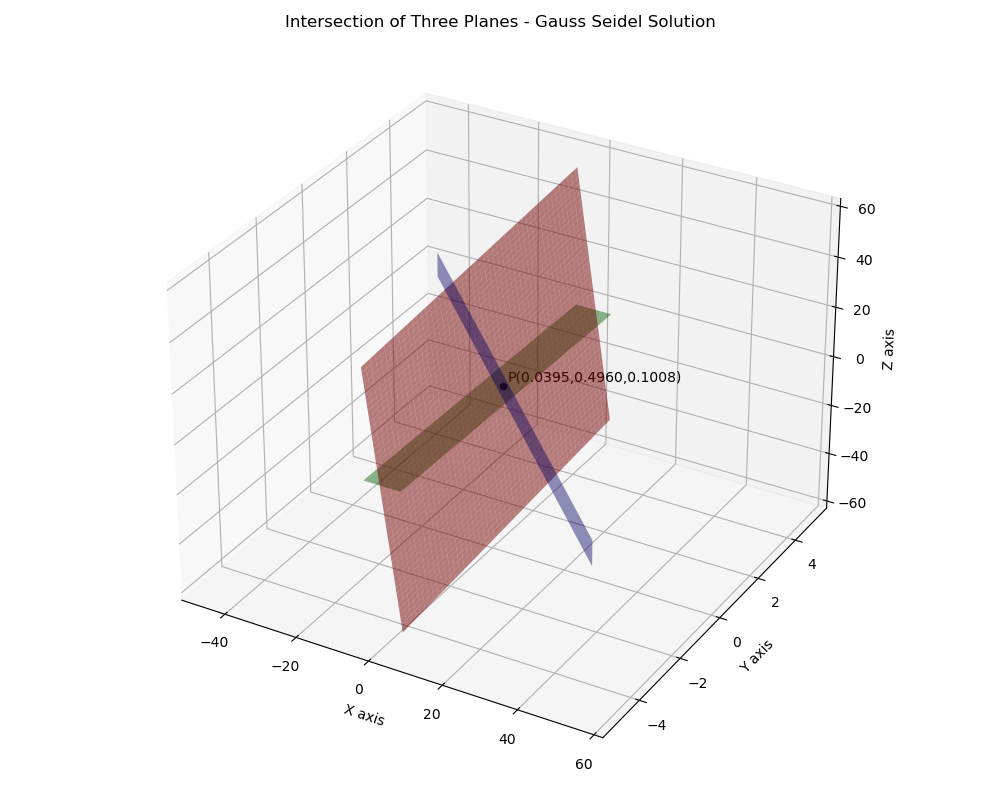
\includegraphics[width=0.8\columnwidth]{figs/solution_gauss_seidel.png} 
   \caption*{Fig : Planes}
  \label{Fig1}
\end{figure}

\end{frame}

\end{document}
